\section{Signal Conditioning}

When a sensor generates an electric signal, that
signal often is either too weak, too noisy, or contains undesirable components. The sensor output may not be compatible with the input requirements of a
data acquisition system, that is, it may have a wrong output format. An interface or a signal conditioning circuit has a specific purpose: to bring
signal from the sensor up to the format that is compatible with the load device.

\begin{figure}[H]
    \centering
    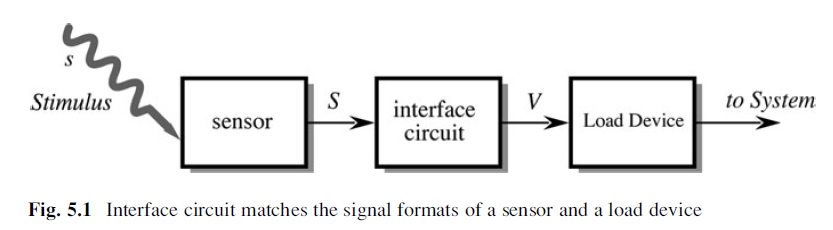
\includegraphics[width = 0.7\textwidth]{L4/img/interface.PNG}
\end{figure}

An example of signal conditioning is the \textbf{voltage attenuation} and the \textbf{current attenuation}.

\begin{minipage}[c]{.45\linewidth}	  
\begin{figure}[H]
    \centering
    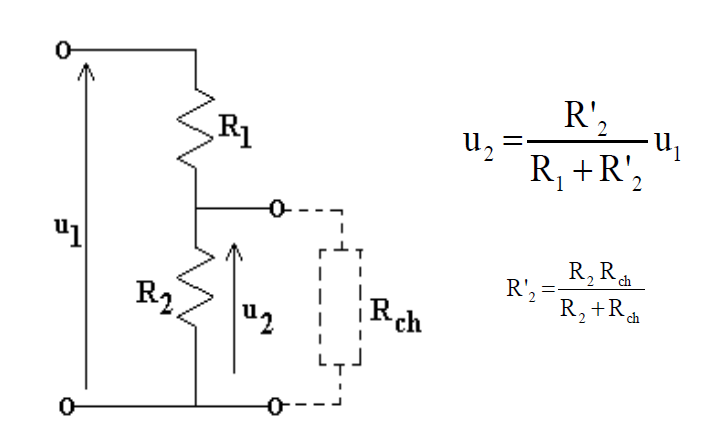
\includegraphics[width = 0.7\textwidth]{L4/img/voltage.PNG}
    \caption{Voltage attenuation}
\end{figure}
\end{minipage} \hfill
\begin{minipage}[c]{.45\linewidth}
   \begin{figure}[H]
    \centering
    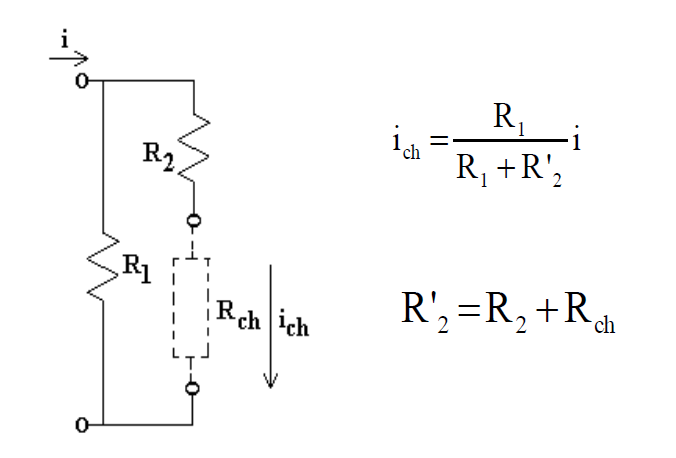
\includegraphics[width = 0.7\textwidth]{L4/img/current.PNG}
    \caption{Current attenuation}
\end{figure}
\end{minipage}

\subsection{Amplifiers and their circuits}

Most passive sensors produce a weak and
noisy signal output in the order of pV or \si{\micro A} and
less. Standard electronics data readers require $\sim$ V
or $\sim$ mA range signal inputs.

As a building block, a good operational amplifier has the following properties:

\begin{itemize}
    \item Two inputs: one inverting (-) and the other is non inverting (+)
    \item A high input resistance of the order of hundreds
of M$\Omega$ or even G$\Omega$
    \item A low output resistance (a fraction of $\Omega$)
    \item The ability to drive capacitive loads
    \item A low input offset voltage $e_0$ (few mV or even \si{\micro V})
    \item A low input bias current $i_0$ (few pA or even less)
    \item A very high \textit{open-loop gain} $A_{OL}$ (at least $10^4$ and
    preferably over $10^6$). The OP AMP must be
    able to magnify (amplify) a voltage difference $V_{in}$
    between its two inputs by a factor of $A_{OL}$.
    \item A high common-mode rejection ratio (CMRR). The amplifier suppresses the in-phase
    equal magnitude input signals (common-mode
    signals) $V_{CM}$ applied to both inputs
    \item Low intrinsic noise
    \item A broad operating frequency range set by the
    product gain-bandwidth (GBW)
    \item A low sensitivity to variations in the power supply
    voltage
    \item A high environmental stability of its own
characteristics
\end{itemize}

\begin{figure}[H]
    \centering
    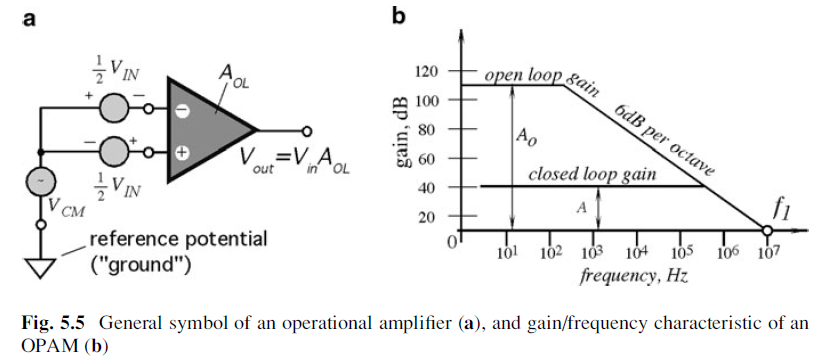
\includegraphics[width = 0.7\textwidth]{L4/img/amp.PNG}
\end{figure}

\subsubsection{Voltage follower}

A voltage follower is a an electronic circuit that provides impedance
conversion from a high to low level. A typical follower has \textbf{high input
impedance} (the high input resistance and the low input capacitance) and \textbf{low output
resistance} (the output capacitance makes no difference). A good follower has a
\textbf{voltage gain very close to unity} (typically 0.999 at lower frequencies) and a high
current gain.

\begin{figure}[H]
    \centering
    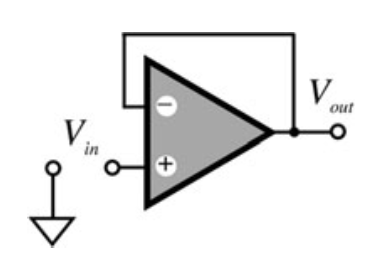
\includegraphics[width = 0.2\textwidth]{L4/img/voltage-follower.PNG}
\end{figure}

\subsubsection{Inverting and non-inverting amplifier}

\begin{minipage}[c]{.45\linewidth}	  
\begin{figure}[H]
    \centering
    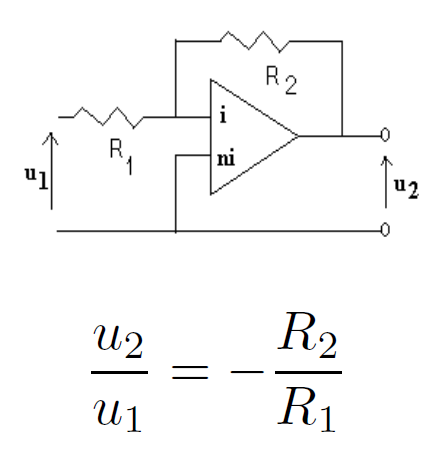
\includegraphics[width = 0.5\textwidth]{L4/img/inverting.PNG}
    \caption{Inverting amplifier}
\end{figure}
\end{minipage} \hfill
\begin{minipage}[c]{.45\linewidth}
   \begin{figure}[H]
    \centering
    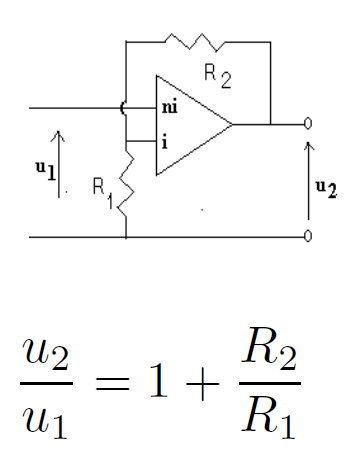
\includegraphics[width = 0.4\textwidth]{L4/img/non-inverting.PNG}
    \caption{Non-inverting amplifier}
\end{figure}
\end{minipage}

With these two configurations, we can build a block performing sums and differences:

\begin{figure}[H]
    \centering
    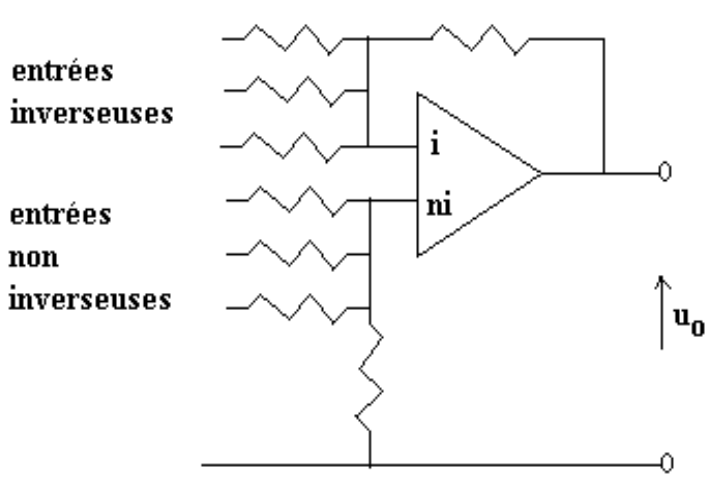
\includegraphics[width = 0.3\textwidth]{L4/img/sum-diff.PNG}
    \caption{Sum and difference}
\end{figure}

\subsubsection{Instrumentation amplifier}

An instrumentation amplifier (IA) has two inputs and one output. It is
distinguished from an operational amplifier by its finite gain (which is usually no
more than 100) and the availability of both inputs to connect to the signal
sources. The latter feature means that all necessary feedback components are
connected to other parts of the instrumentation amplifier, rather than to its non inverting
and inverting inputs. The main function of the IA is to produce an output
signal which is proportional to the difference in voltages between its two inputs:

$$V_{out} = a(V_+ - V_-) = a \Delta V$$

\begin{figure}[H]
    \centering
    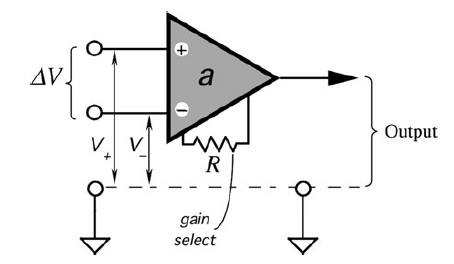
\includegraphics[width = 0.4\textwidth]{L4/img/instr-amp1.PNG}
\end{figure}


\begin{itemize}
    \item Particularly useful for measuring floating voltages because no need to be connected to the GND
   \item Limited but calibrated
    and programmable gain $\approx$ 100
    \item High input impedance
    \item High common-mode
    rejection ratio (CMRR):
    $\dif\: V_{out}/\dif\: (V_++V_-)$
    \item High power supply rejection
    ratio: $\dif\: V_{out}/\dif\: V_{DD}$
    \item Low offset:
    $\Delta$V generating $V_{out}=0$
\end{itemize}
A classical implementation of an IA is composed of 3 operational amplifiers as follows. The gain $a$ is adjusted by the value of $R_3$.

\begin{figure}[H]
    \centering
    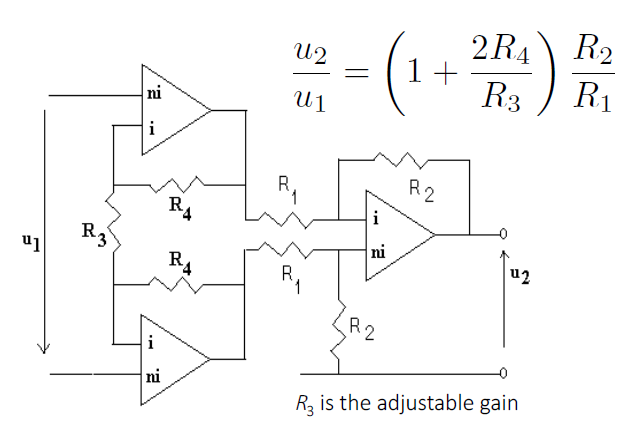
\includegraphics[width = 0.5\textwidth]{L4/img/instr-amp2.PNG}
\end{figure}

\subsubsection{Charge amplifier}

Charge amplifiers are configured as charge to voltage or as current to voltage converters.
It is interesting for piezoelectric sensors, which is a passive capacitive sensor, it directly converts a stimulus into an electric charge or current. On configuration a, we have an integrator, the output voltage is thus proportional to the change of charge $\Delta Q$.

\begin{figure}[H]
    \centering
    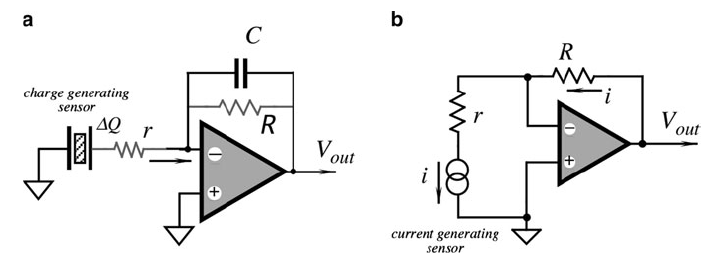
\includegraphics[width = 0.6\textwidth]{L4/img/charge-amp.PNG}
\end{figure}

\subsubsection{Light-to-voltage converter}

Light-to-voltage converters are based on combination of photosensors and current to
voltage converter circuits. For detecting extremely low-intensity light, typically
one or several photons, the \textbf{photomultipliers} are generally employed (fragile/expensive).
However, for less demanding applications three types of photosensors are available:
a photodiode, phototransistor, and photoresistor. Here we take interest in \textbf{photodiode}.

From the electrical point of view, a photodiode can be represented by an
equivalent circuit. It consists of a current generator (internal
input impedance is infinitely large), a parallel regular diode (like a rectifier diode),
resistance of the junction $R_j$, capacitance of the junction $C_j$, and a serial resistance
$R_s$. The current generator generates a photocurrent proportional to the photon flux.
This current flows in the direction from the cathode (-) to the anode (+) of the
photodiode. Note that for very strong illuminations, the photocurrent will start
flowing through a nonlinear rectifier diode, which will degrade a linearity. To have a good linearity, we have to work in the \textbf{reverse biased zone}. We use the circuit of Figure b to move the characteristic of the resistance (doted line in Figure c) on the left.

\begin{figure}[H]
    \centering
    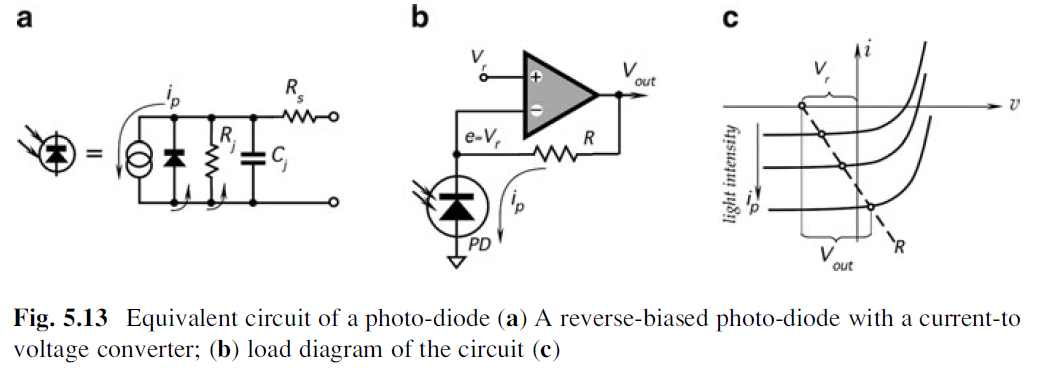
\includegraphics[width = 0.8\textwidth]{L4/img/photodiode.PNG}
\end{figure}

A photodiode can be used in \textbf{voltaic} or \textbf{current} modes. In the voltaic mode, a
photodiode is connected to a very high resistor. The diode will work like a battery with voltage proportional to the light intensity. This voltage is the result of a photocurrent $i_p$ passing through the internal
junction resistance $R_j$. In a current mode, the photodiode is virtually shorted
(a voltage across the diode is zero) and current $i_p$ is drawn to the current-to-voltage
converter as described in the above schematic. 


\paragraph{Light-to-voltage with zero-biased photodiode}

An arrangement with no
bias and high-impedance loading to the photodiode provides less influence by dark
current and a wide linear range of the photocurrent relative to the radiant intensity.

\begin{figure}[H]
    \centering
    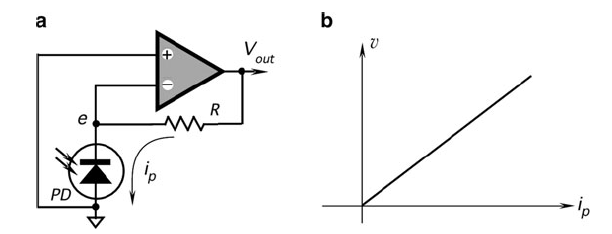
\includegraphics[width = 0.4\textwidth]{L4/img/zero-biased.PNG}
\end{figure}

\subsubsection{Schmitt Trigger}

A Schmitt trigger is a comparator circuit with hysteresis. It is an active circuit which converts an analog input signal to a digital output signal. When the input is higher than a chosen threshold, the output is high. When the input is below a different (lower) chosen threshold the output is low, and when the input is between the two levels the output retains its value. This dual threshold action is called hysteresis.

This configuration is useful to get rid of noise. If the noise doesn't reach the threshold, the output does not go high or low.

\begin{figure}[H]
    \centering
    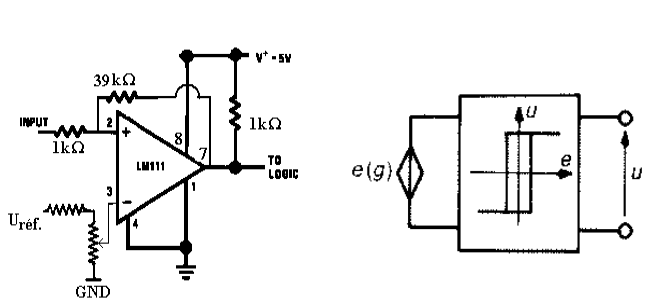
\includegraphics[width = 0.6\textwidth]{L4/img/schmitt.PNG}
\end{figure}

\subsection{Filters}

\subsubsection{First order filters}

\begin{figure}[H]
    \centering
    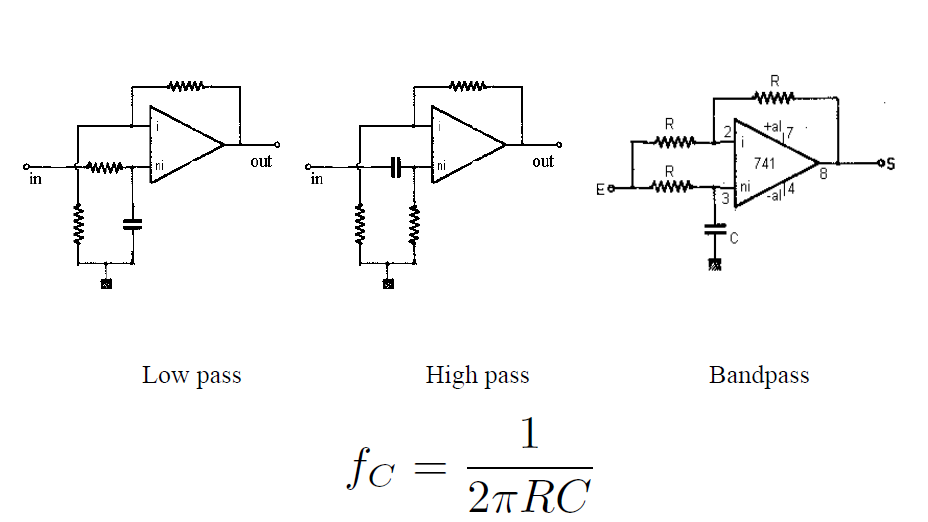
\includegraphics[width = 0.7\textwidth]{L4/img/first-order-filters.PNG}
\end{figure}

For instance, the following results state for a first order low-pass filter:

\begin{eqnarray}
I &=& \dfrac{V_{in}}{R + \dfrac{1}{j\omega C}} \\
V_{out} = I\cdot \dfrac{1}{j\omega C} &=& \dfrac{V_{in}}{R + \dfrac{1}{j\omega C}} \cdot \dfrac{1}{j\omega C} \\
 &=& \dfrac{V_{in}}{j\omega RC + 1} = \dfrac{V_{in}}{j(f/f_c) + 1}
\end{eqnarray}

The same kind of result can be found for a first order high-pass filter. 

\subsubsection{Second order filters}

\paragraph{Low pass filter}:

\begin{figure}[H]
    \centering
    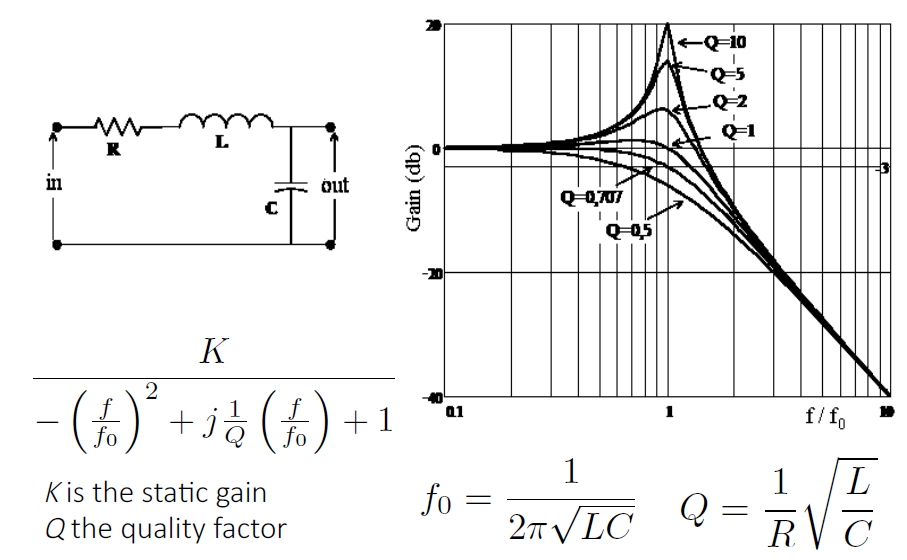
\includegraphics[width = 0.6\textwidth]{L4/img/2nd-LP.PNG}
\end{figure}


\paragraph{High pass filter}:

\begin{figure}[H]
    \centering
    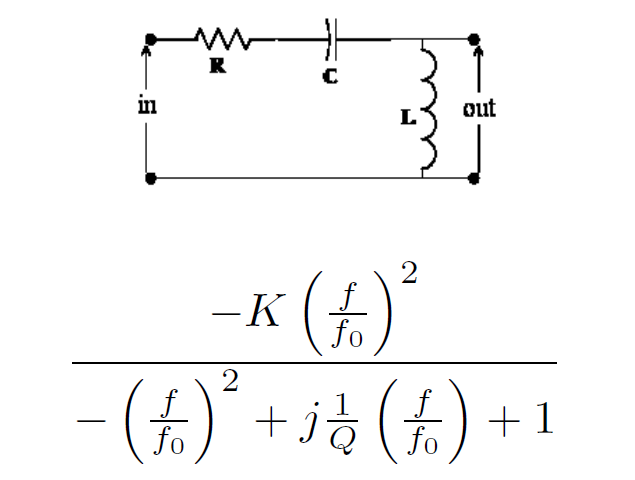
\includegraphics[width = 0.5\textwidth]{L4/img/2nd-HP.PNG}
\end{figure}

Disadvantage : if we measure close to the overshoot, the noise could affect a lot the measurement, which is not what we want. Thus, we have to reduce the quality factor $Q$ if we want to measure a value in a wide range of frequencies. $f_0$ is the resonance frequency.

For both cases, we can make the analogy between the quality factor $Q$ and the damping factor $m$ as following:

$$\dfrac{1}{Q} = 2 m$$

Moreover, we can say that
\begin{itemize}
    \item if $m \geq 1$ then $f_0$ is the cut-off frequency
    \item if $m< 1$ then $f_0$ is the resonance frequency
\end{itemize}

\textbf{Sallen-Key} filters were used in the light sensing circuits.

\subsection{DC Bridges}

\subsubsection{Differential sensing}

The differential sensing aims at cancelling additive and environmental noise by subtracting the real signal $S_1$ and the reference signal $S_0$. This reference signal is produced by a reference sensor that is isolated from the physical input
stimuli. This technique is effective against common-mode noise because the noise has the same amplitude and phase. It is also characterized by a common-mode rejection ratio that has to be as small as possible: $CMRR = 0.5\frac{S_1 + S_0}{S_1 - S_0}$.

\begin{figure}[H]
    \centering
    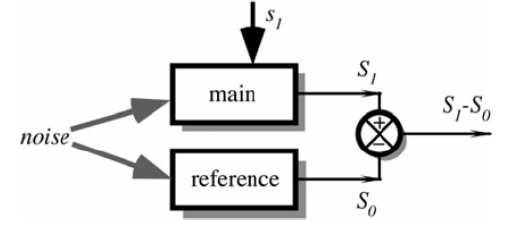
\includegraphics[width = 0.5\textwidth]{L4/img/diff-sensing.PNG}
\end{figure}

\subsubsection{Ratiometric sensing}

This technique is used to cancel multiplicative
environmental noise. For example, cancelling of temperature variations:

$$ V_1 = [1+ \alpha(T - T_0)]f(s_1) $$
$$ V_2 = [1+ \alpha(T - T_0)]f(s_2) $$

$$\rightarrow \frac{V_1}{V_0} = \frac{f(s_1)}{f(s_2)}$$

\subsubsection{Wheatstone Bridge}

A Wheatstone bridge is both differential and ratiometric. It allows to eliminate the effect of an influencing parameter, such
as the temperature (multiplicative noise). It presents a \textbf{double sensitivity} and a lower dependance with respect to the
supply voltage variation compared to the simple attenuator.
\begin{figure}[H]
    \centering
    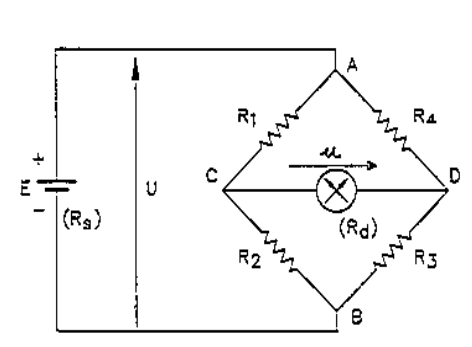
\includegraphics[width = 0.3\textwidth]{L4/img/wheatstone.PNG}
\end{figure}
In this kind of circuit, $u=0$ means that the circuit is equilibrated/null-balanced. This implies that 
$$ R_1 R_3 = R_2 R_4 $$ 
This behaviour allows for example to measure one of the four resistance values if we know precisely the three other ones.
The main advantages of using a Wheatstone bridge are the following:
\begin{itemize}
    \item The voltage supply is only influencing the sensitivity, there is no impact of
its stability
    \item Only its resolution matters, the precision of the detector has no influence since $u$ is kept to zero by changing another resistance (such as $R_2$) 
\end{itemize}
Let us have $ R_3 = R_{3,0} (1+\rho) = R_{3,0} + \rho R_3$. The sensitivity of the Wheatstone bridge is given by $u = \frac{\rho E}{2 + \frac{R_1}{R_2} + \frac{R_2}{R_1}}$(considering $R_d$ infinite). Moreover, the optimum sensitivity is obtained for $R_1=R_2$ and $R_3=R_4$, which leads to $$ u_{opt} = \frac{\rho E}{4} $$ with $\rho = \delta \mathbf{Z_3}/\mathbf{Z_3}$. Thus, $\rho$ is a percentage of increment of the initial value of the resistance. 

\paragraph{Disbalanced bridge}:

\begin{minipage}[c]{.45\linewidth}	  
\begin{figure}[H]
    \centering
    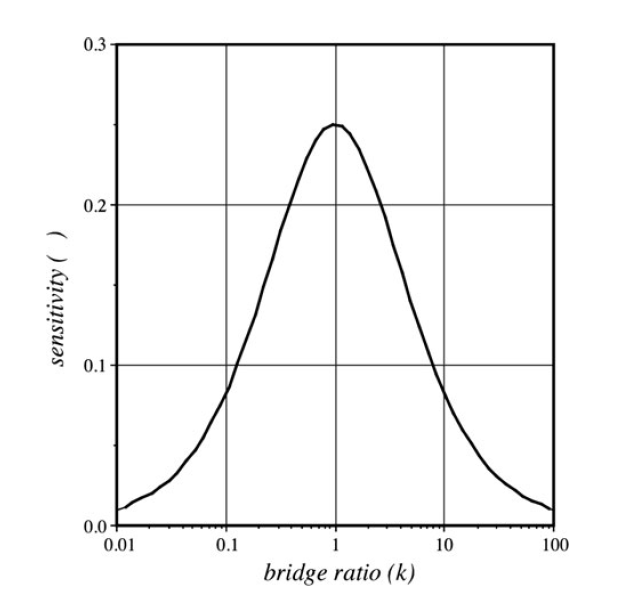
\includegraphics[width = 0.7\textwidth]{L4/img/disbalanced.PNG}
\end{figure}
\end{minipage} \hfill
\begin{minipage}[c]{.45\linewidth}
A basic Wheatstone bridge circuit generally operates with a disbalanced
bridge ($R_1 \ne R_2$). This is called the deflection method of measurement. It is based on
 detecting the voltage across the bridge diagonal. The bridge output voltage is a nonlinear function of a disbalance $\rho$, where the sensor resistance is $R_3 = R_{3,0}(1 + \rho)$.

The graph indicates that the maximum sensitivity is achieved for $k=1$. However, the
sensitivity drops relatively little for the range where $0.5 < k < 2$.
\end{minipage}

\paragraph{Null-balanced bridge}

Another method of using a bridge circuit is called a null-balance. The method
overcomes the limitation of small changes in the bridge arm to achieve a good
linearity. The null-balance essentially requires that the bridge is always maintained
at the balanced state. A control circuit modifies the value of $R_4$ on a command from an error
amplifier.
    
\paragraph{Bridge for high resistance}

It has a lowered sensitivity since $R_d$
cannot be neglected.
The voltage can be increased as the current passing through the high resistances is small.
One trick is to use $R_2$ and $R_3$
with lower values than $R_1$ and
$R_4$ so that the detector remains
at a low potential.
The sensitivity is also lowered
using this trick.

\subsection{AC Bridges}

\subsubsection{Impedance bridge}

\begin{figure}[H]
    \centering
    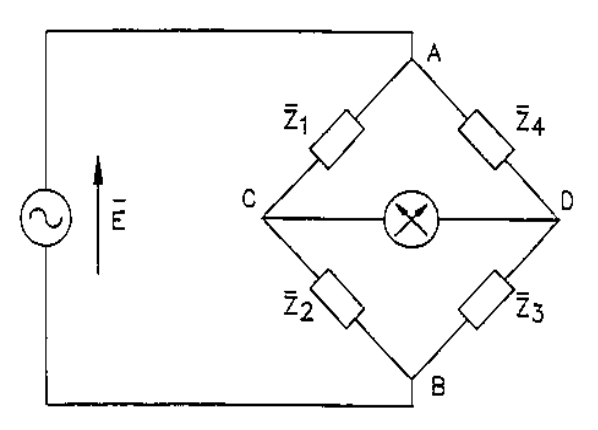
\includegraphics[width = 0.4\textwidth]{L4/img/impedance-bridge.PNG}
\end{figure}

The bridge is equilibrated when $Z_1 Z_3 = Z_2 Z_4$. The advantages are similar to the DC bridge. 

\subsubsection{Maxwell bridge}

\begin{minipage}[c]{0.45 \linewidth}
\begin{figure}[H]
    \centering
    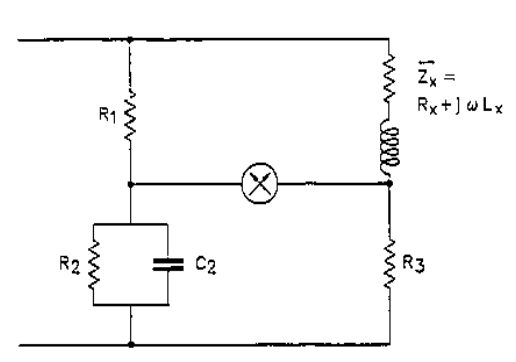
\includegraphics[width = 0.7\textwidth]{L4/img/maxwell-bridge.PNG}
\end{figure}
\end{minipage}\hfill
\begin{minipage}[c]{0.45 \linewidth}
To have an equilibrated circuit, we need

$$ R_x + j\omega L_x = R_1 R_3 \left(\frac{1}{R_2} + j \omega C_2\right) $$

Therefore,

$$ L_x = R_1 R_3 C_2 $$
$$ R_x = R_1 R_3/R_2 $$

The equilibrium is thus independent of the frequency at which we solicit the bridge (less impact of the harmonics).
\end{minipage}


\subsubsection{Hay bridge}

\begin{minipage}[c]{0.45 \linewidth}
\begin{figure}[H]
    \centering
    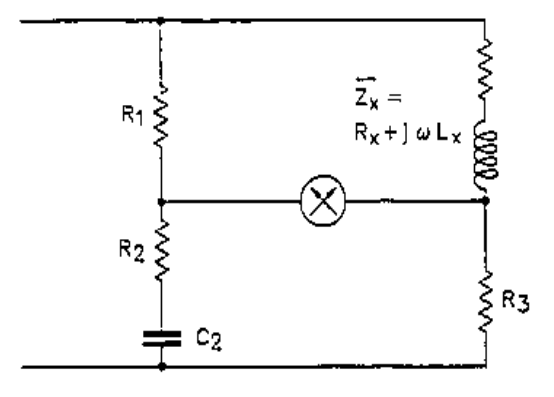
\includegraphics[width = 0.7\textwidth]{L4/img/hay-bridge.PNG}
\end{figure}
\end{minipage}\hfill
\begin{minipage}[c]{0.45 \linewidth}
    If we develop the equilibrium condition, we will observe that the equilibrium is frequency dependant.
\end{minipage}

\subsubsection{Owen bridge}

\subsubsection{Wien bridge}


\begin{minipage}[c]{0.45 \linewidth}
\begin{figure}[H]
    \centering
    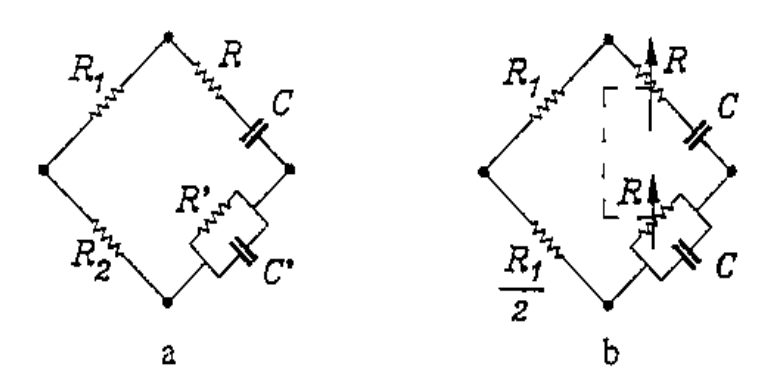
\includegraphics[width = 0.7\textwidth]{L4/img/wien-bridge.PNG}
\end{figure}
\end{minipage}\hfill
\begin{minipage}[c]{0.45 \linewidth}
    The equilibrium is strongly dependant upon the frequency, it is thus used for frequency measurement or as sine oscillator with an op amp.
    
\textbf{Remark}: the right branch is also used as bandpass filter. This bridge has a good resolution.
\end{minipage}

\subsubsection{Sensitivity of impedance bridges}

Let us assume that $\overline{\rho} = \dif \overline{Z}/\overline{Z}$, we get $$ \overline{u} = \frac{\overline{\rho} \overline{E}}{2 + \overline{a} + 1/ \overline{a}} $$
with $\overline{a} = \frac{\overline{Z_1}}{\overline{Z_2}} = a e^{j\theta}$.
If we act on the amplitude $a$ without changing the phase $\theta$,
the sensitivity is maximum for $a = 1$. The sensitivity is then $$|\overline{u}|_{max} = \frac{\rho E}{2(1+cos \theta)}$$
AC bridges are better than DC bridges since $\cos \theta < 1$. Indeed, 
$$|\overline{u}|_{max} = \frac{\rho E}{2(1+cos \theta)} > u_{opt} = \frac{\rho E}{4}  $$
If we act on the phase $\theta$ without changing the amplitude $a$, the
maximum sensitivity is obtained for $\theta = \pm \pi$ and we get:
$$ |\overline{u}|_{max} = \frac{\rho a E}{(1-a)^2} $$ 
At last, if we act on both parameters, the maximum sensitivity
is obtained for the following condition:
$$ a=1 \text{ and } \theta = \pm \pi  $$
and the sensitivity is (theoretically) infinite.

\subsection{Oscillators}

There are two types of oscillator:

\begin{itemize}
    \item Sine oscillators (unstable linear circuit)
    \item Binary oscillators (strongly non linear)
\end{itemize}
Sine oscillators are often composed of two
opposite reactances (such as capacitance +
inductance).
The oscillators can be used as impedance-to-frequency converters. 
A bad oscillator shifts the frequency over time. A good inductance corresponds to a good oscillator.

\subsubsection{Quartz oscillator}

\begin{figure}[H]
    \centering
    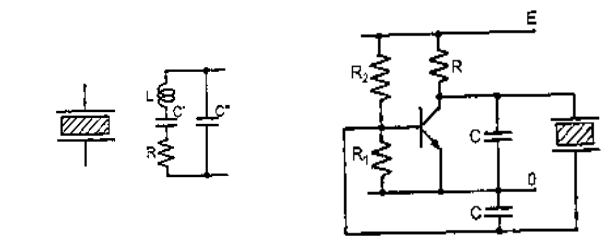
\includegraphics[width = 0.6\textwidth]{L4/img/quartz-oscillator.PNG}
\end{figure}

Quartz oscillator are cheap, precise and stable with temperature. It gives a time reference such as in quartz clock watches or in clock of a computer.
The difficult part is to avoid operating on the harmonics.
This can be avoided by inserting the quartz (little box in the circuit) in an LC circuit to force the desired harmonic. 

\subsection{Capacitance to voltage: the accelerometer}

It is characterized by a second order transfer function and thus has a natural frequency $f_n$. The reference frequency $f_{ref}$ is the main frequency at which the accelerometer is operating.
